
\section{The Frequency Domain}

\begin{frame}{Simple Frequency Decomposition}
	\begin{figure}
		% Source - https://tex.stackexchange.com/q/127375
		% Posted by Shuhao Cao, modified by community. See post 'Timeline' for change history
		% Retrieved 2026-08-13, License - CC BY-SA 3.0
		
		$y(t) =  2.2 \sin(10t)  + \sin(22t )$
		
		\vspace{1.0cm}
		
		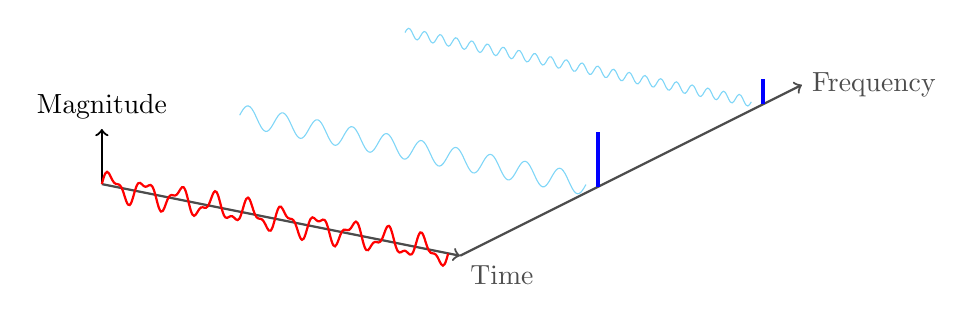
\begin{tikzpicture}[x={(1cm,0.5cm)},z={(0cm,0.5cm)},y={(1cm,-0.2cm)},scale=0.70]
			\draw[->,thick,black!70] (0,6.5,0) -- (6.2,6.5,0) node[right] {Frequency};
			\draw[->,thick,black!70] (0,0,0) -- (0,6.5,0) node[below right] {Time};
			\draw[->,thick] (0,0,0) -- (0,0,2) node[above] {Magnitude};
			\foreach \y in {2.5,5.5}{
				\draw [cyan!50, domain=0:2*pi,samples=200,smooth] 
				plot (\y,\x, {sin(4*\y*\x r)/\y });
				\draw[blue, ultra thick] (\y,6.5,0) -- (\y,6.5,5/\y);
			}
			\draw [red, thick, domain=0:2*pi,samples=200,smooth] 
			plot (0,\x, {0*sin(4*0.5*\x r)/0.5 + 0*sin(4*1.5*\x r)/1.5 + 1*sin(4*2.5*\x r)/2.5 + 0*sin(4*3.5*\x r)/3.5 + 0*sin(4*4.5*\x r)/4.5 + 1*sin(4*5.5*\x r)/5.5} );
		\end{tikzpicture}
		\caption{Simple signal represented in both time and frequency domains}
	\end{figure}
\end{frame}

\begin{frame}{Square Frequency Decomposition}
	\begin{figure}
		% Source - https://tex.stackexchange.com/q/127375
		% Posted by Shuhao Cao, modified by community. See post 'Timeline' for change history
		% Retrieved 2026-08-13, License - CC BY-SA 3.0
		
		\[
		y(t) =
		\frac{4}{\pi}
		\sum_{k=0}^{\infty}
		\frac{1}{2k+1}
		\sin\left((2k+1)\omega_0t\right)
		\]
		
		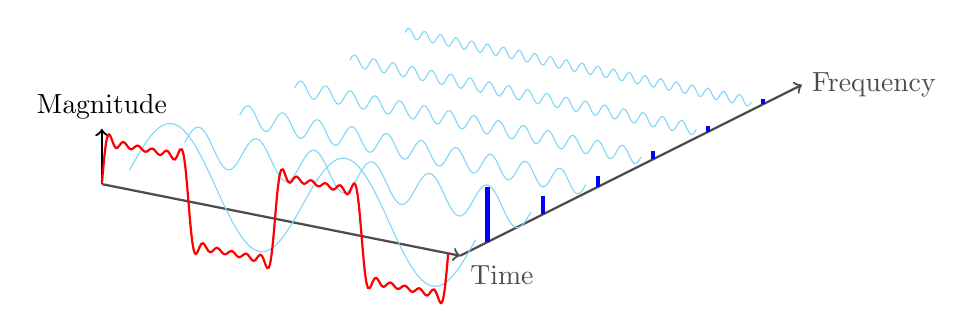
\begin{tikzpicture}[x={(1cm,0.5cm)},z={(0cm,0.5cm)},y={(1cm,-0.2cm)},scale=0.70]
			\draw[->,thick,black!70] (0,6.5,0) -- (6.2,6.5,0) node[right] {Frequency};
			\draw[->,thick,black!70] (0,0,0) -- (0,6.5,0) node[below right] {Time};
			\draw[->,thick] (0,0,0) -- (0,0,2) node[above] {Magnitude};
			\foreach \y in {0.5,1.5,...,5.5}{
				\draw [cyan!50, domain=0:2*pi,samples=200,smooth] 
				plot (\y,\x, {sin(4*\y*\x r)/\y });
				\draw[blue, ultra thick] (\y,6.5,0) -- (\y,6.5,1/\y);
			}
			\draw [red, thick, domain=0:2*pi,samples=200,smooth] 
			plot (0,\x, {sin(4*0.5*\x r)/0.5 + sin(4*1.5*\x r)/1.5 + sin(4*2.5*\x r)/2.5 + sin(4*3.5*\x r)/3.5 + sin(4*4.5*\x r)/4.5 + sin(4*5.5*\x r)/5.5} );
		\end{tikzpicture}
		\caption{Square wave signal represented in both time and frequency domains}
		\url{tex.stackexchange.com/q/127375}
		
	\end{figure}
\end{frame}

\begin{frame}{Euler Equation}
	\begin{figure}
		
		Any complex number can be represented as a complex exponential.
		\begin{align*}
			e^{i\omega t} = \cos(\omega t) + i\sin(\omega t)
		\end{align*}
		
		Multiplying complex numbers and complex exponentials together is like shifting the phase of a sine wave, especially when using conjugated weights and negative frequencies. More on this later...
		\begin{align*}
			(A+iB) e^{i\omega t} + (A-iB) e^{-i\omega t} &=2A \cos(\omega t) - 2B \sin(\omega t) \\ 
			&= C \cos(\omega t + \phi)  \\ 
		\end{align*}
	\end{figure}
\end{frame}

\begin{frame}{Discrete Fourier Transform}
	\begin{figure}
		\begin{align*}
		\mathbf{X} &= 	\mathcal{F}\{\mathbf{x}\} \\
		X[k] &= \sum_{n=0}^{N-1} x[n] e^{-i\frac{2\pi}{N}kn},
		\qquad k=0,1,\ldots,N-1 \\
		\begin{bmatrix}
			X[0]\\
			X[1]\\
			X[2]\\
			\vdots\\
			X[N-1]
		\end{bmatrix}
		&=
		\begin{bmatrix}
			1 & 1 & 1 & \cdots & 1\\
			1 & e^{-i\frac{2\pi}{N}} & e^{-i\frac{4\pi}{N}} & \cdots & e^{-i\frac{2\pi(N-1)}{N}}\\
			1 & e^{-i\frac{4\pi}{N}} & e^{-i\frac{8\pi}{N}} & \cdots & e^{-i\frac{4\pi(N-1)}{N}}\\
			\vdots & \vdots & \vdots & \ddots & \vdots\\
			1 & e^{-i\frac{2\pi(N-1)}{N}} &
			e^{-i\frac{4\pi(N-1)}{N}} &
			\cdots &
			e^{-i\frac{2\pi(N-1)^2}{N}}
		\end{bmatrix}
		\begin{bmatrix}
			x[0]\\
			x[1]\\
			x[2]\\
			\vdots\\
			x[N-1]
		\end{bmatrix} \\
		\mathbf{X} &= \mathbf{F}_N \mathbf{x}
		\end{align*}
	\end{figure}
\end{frame}

\begin{frame}{Example Chirp}
	\centering
	\begin{align*}
		sinc(t) &= \frac{sin(t)}{t} \\
		\mathcal{F}\{sinc(t)\} &= rect(\omega)
	\end{align*}
	\begin{columns}
		\begin{column}{0.48\textwidth}
			\centering
			\includegraphics[width=\linewidth]{../../python_correlation_sandbox/modern/saved_figs/00_sinct_10hz.pdf}
%			\captionof{figure}{$sinc(t)$}
		\end{column}
		\begin{column}{0.48\textwidth}
			\centering
			\includegraphics[width=\linewidth]{../../python_correlation_sandbox/modern/saved_figs/01_freq_mag_of_sinct_10hz.pdf}
%			\captionof{figure}{Second Caption}
		\end{column}
	\end{columns}
\end{frame}


\begin{frame}{Key Point - DFT Is A Matrix Multiplication}
		\begin{block}{Key Idea}
				The Discrete Time Fourier Transform (DFT) can be represented as a matrix multiplication.
			\end{block}
		
%		\vspace{0.3cm}
%		
%		\begin{alertblock}{Important}
%				The Discrete Time Fourier Transform (DFT) can be represented as a matrix multiplication.
%			\end{alertblock}
	\end{frame}